%                                                                 aa.dem
% AA vers. 8.2, LaTeX class for Astronomy & Astrophysics
% demonstration file
%                                                       (c) EDP Sciences
%-----------------------------------------------------------------------
%
%\documentclass[referee]{aa} % for a referee version
%\documentclass[onecolumn]{aa} % for a paper on 1 column  
%\documentclass[longauth]{aa} % for the long lists of affiliations 
%\documentclass[rnote]{aa} % for the research notes
%\documentclass[letter]{aa} % for the letters 
%\documentclass[bibyear]{aa} % if the references are not structured 
% according to the author-year natbib style

% V3

%
\documentclass{/Users/art2/TeX/aanda/aa} 
%\documentclass[referee]{/Users/art2/TeX/aanda/aa} 
%\documentclass{aa}
%\documentclass{article}
%
%\usepackage{graphicx}
\usepackage{graphicx}
%\usepackage{psfig}
%%%%%%%%%%%%%%%%%%%%%%%%%%%%%%%%%%%%%%%%
\usepackage{txfonts}
%\usepackage{longtable}
%%%%%%%%%%%%%%%%%%%%%%%%%%%%%%%%%%%%%%%%
\bibpunct{(}{)}{;}{a}{}{,} % to follow the A&A style
%\usepackage[options]{hyperref}
% To add links in your PDF file, use the package "hyperref"
% with options according to your LaTeX or PDFLaTeX drivers.

\def\kms {km\,s$^{-1}$}

\setlength{\LTcapwidth}{16cm}
\begin{document} 


   \title{Making sense of Betelgeuse and other RSG spectra\thanks{Based on observations obtained at the T\'elescope Bernard Lyot
(TBL) at Observatoire du Pic du Midi, CNRS/INSU and Universit\'e de
Toulouse, France.}}
   %\subtitle{Velocities}

   \author{{ A.~L{\'o}pez Ariste}\inst{1}, { Q.~Pilates}\inst{1},{ A.~Lavail}\inst{1},{ Ph. Mathias}\inst{1},  }
   \date{Received ...; accepted ...}

   
   \institute{IRAP, Universit\'e de Toulouse, CNRS, CNES, UPS.  14, Av. E. Belin. 31400 Toulouse, France 
%\institute{IRAP - CNRS UMR 5277. 14, Av. E. Belin. 31400 Toulouse. France 
  %  \and Universit\'e de Toulouse, UPS-OMP, Institut de Recherche en Astrophysique et Plan\'etologie, Toulouse, France}
}

% \abstract{}{}{}{}{} 
% 5 {} token are mandatory
 
  \abstract
  % context heading (optional)
  {}
  % {} leave it empty if necessary  
   {}
  % aims heading (mandatory)
   {}
  % methods heading (mandatory)
   { }
     % results heading (mandatory)
   {}
  % conclusions heading (optional), leave it empty if necessary 
  
   \keywords{}

\titlerunning{Making sense of RSG spectra}
\authorrunning{A. L\'opez Ariste et al.}

   \maketitle
%

\section{The issue with RSG spectra.}
The discovery of linear polarisation in the atomic lines of the spectrum of Betelgeuse \cite{}  opened the path to a succesful imaging technique 
that has provided continuous images of the convective structures in the photosphere of Betelgeuse (since 2013) and other RSGs. More recently, exploiting 
the different formation heights of different atomic lines, 3-dimensional images of the photosphere have been inferred from those spectropolarimetric 
signals. Beyond the images themselves, this technique has unveiled the large convective velocities predicted by numerical simulation codes and confirmed 
the size and temporal scale of variation of these convective structures. The measurement of plasma velocities at different heights has also uncovered 
plasma plumes that barely change velocity as they rise through the atmosphere of Betelgeuse, pointing to the presence of an acceleration mechanism 
hitherto unidentified but present from the photospheric heights and able to equilibrate forces with gravity and maintain plasma velocities as 
they approach the height at which the will definitely escape as stellar wind.

These successes were founded in a series of approximations about the polarized line formation which have been discussed and partially justified 
on the cited literature. Among them, perhaps the weakest is the imposition of a relationship between brightness and vertical velocity. Such correlation 
is observed whenever line formation happens while convection is still the dominat dynamical process, as in the Sun. Numerical simulations of the 
photosphere of Betelgeuse appear to infirm such relationship and suggest that the line formation region resides above the convective zones, and brightness 
and velocity would not be clearly correlated in the formation of spectral lines in Betelgeuse. Against this prediction stands the comparison of 
images inferred from spectropolarimetry assuming this correlation true and the images taken by interferometry. 

\cite{} explored whether convection still leaves a signature in the intensity spectra and, through a newly-developed tomographic technique, unveiled 
a histeresis loop reminiscent of what could be expected if lines were formed in convective conditions, when the correlation of brightness and 
vertical velocities is still valid. Such histeresis loops could be seen in observed spectra and also, marginally, in synthetic spectra computed 
by radiative transfer through stellar snapshot from numerical simulations. But these same authors claimed that such histeresis loops may be understood 
not as reflecting that lines form where convection takes place, but rather that acoustic waves or pulsation may propagate correlations of the 
kind to selected patches well above where convection dominates and where atomic lines form. 
Since, traditionally, convection has also been called for to explain the C-shape line asymmetries, it should go without further justification that 
it is in the intensity profile that we should seek the answer to the validity of the brightness-velocity correlation at the core of the interpretation
of the measured linear polarization in terms of images of convective structures. 

However, inspection of the observed intensity and linear polarization profiles makes it clear that there is a further problem with intensity profiles 
than just correctly interpreting bisectors or hysteresis loops. As emphasized by who?, the intensity profiles observed on Betelgeuse are astonishingly 
narrower than the width of the linear polarization signal. This is illustrade once again in Fig. 1, where the limits of $v_0$ the assumed velocity 
of the star, and $v_{max}$, the assumed highest velocity of the rising plasma are also shown. These two limits are set by simple inspection of the
accumulated data set of linear polarization profiles. In a model of pure convective movements, all that is bright is rising vertically, and the most 
blushifted signal observed must come from plasma rising at exactly disk center at the maximum velocity possible. Thus, no linear polarization is 
to be observed at shorter wavelengths than this $v_{max}$ limit. Similarly, plasma at the limb of the star emits at zero velocity respect to the 
bulk star's velocity $v_0$. This red limit is not strict, sinking plasma, though darker than rising plasma, produces signals redder than this limit. And 
\cite{} interpreted the spectra of the RSG $\mu $Cep as the intermittent plumes arising in the back hemisphere of the star, but rising high enough to 
be visible above the limb.  \cite{} discussed at length the validity and justification of the assumed limits for Betelgeuse.  In what concerns here, nevertheless, 
it is most obvious that whatever the precise value of $v_{max}$, there is a considerable amount of linear polarization arising from the continuum beyond the blue 
wing of the line seen in intensity. This is just nonsense. Continuum is precisely defined by its quasi-independence of wavelength, at least at the 
scales here concerned. This linear polarization cannot be due to any continuum emitting process. Interpreting it as the polarisation of the extreme 
wing of the spectral line makes no much sense either. It would require polarisation levels of 10\% at some moments, which is also nonsense. There is no 
mechanism by which such high levels of linear polarization can be created in the extreme wing of the line, when elsewhere in the line the observed amplitudes 
are in the 0.1\% range at most. 

This is the problem we address in the present work. We propose a mechanism by which the intensity line, after integration over the disk, is narrowed 
while the linear polarisation profile keeps the original width. Such mechanism is based upon two ingredients. The first one is  the integration over the disk gives 
weight to signals emerging from the disk center, beceause the wavelength of emission is modulated by its projection onto the line of sight, and the
$\cos \theta$ function reaches a maximum at disk center, hence velocities at disk center, if relatively homogeneous, add up together, while at 
the limb a small change in position changes the projected velocity, even if the atmosphere is homogeneous. This effect is common to all disk integrations, so, alone, 
it makes no difference between Betelgeuse and any other star. The second ingredient is critical: it requires the presence of gradients of velocity 
in the region of formation of the line larger than the widht of the local line. These gradients deformate the line profiles giving them a triangular 
shape. Due to it, and in a nutshell: regions at disk center with large gradients produce  triangular shape profiles contribute to all wavelengths, while 
regions at the limb with low gradients produce narrow gaussian profiles at near zero velocities. The correct addition of these contributions 
produces the observed profiles as we shall demonstrate in the next section. 

In the process to understand the intensity profiles of Betelgeuse, it has been a key element the observation of another RSG, RW Cep. This star 
is not particularly different than Betelgeuse or any other well classified RSG. Any differences between Betelgeuse and RW Cep, as with any other star 
must be mostly attributed to whatever the star is doing right now: is it quietly convecting as Betelgeuse appears to do (except perhaps during 
the recent great dimming event), or is it in a Decin stage as $\mu$ Cep, with repeated events of large plumes raising sufficiently high to escape 
gravity and form a new shell of dust clumps. It was a big surprise to discover therefore that RW Cep presents in our 2023 observations a large and 
broad profile, fully compatible with the linear polarisation signals and unlike anything observed in Betelgeuse in the last 10 years. RW Cep is 
doing something right now which broadens the profiles. Atmospheric dynamics, in its most broad sense, are therefore able to broaden or narrow intensity 
profiles. The narrow profiles are not intrinsic to an RSG, they are rather due to the present dynamics of the star. This realisation opened the path 
to our proposed solution. In Section 3 we explore how our proposition based upon velocity gradients can explain both Betelgeuse and RW Cep intensity 
profiles.

Two last observational facts are discussed and modelled in Section 4. Bisectors of Betelgeuse line profiles often present a typical C-shape, but 
from time to time they reverse their asymmetry. When looking into lines formed in particular regions, the situation appears clearer in that deep 
lines (meaning lines forming deep in the photosphere) present systematically a C-shape bisector, while high lines present a reverse-C bisector. When
adding them together, it will depend on the differential brightness of high to deep lines that the compund spectral line presents one or to other asymmetry.
Our proposed solution must explain these differences and their change in time. And finally, the intensity line presents a velocity span of 7-10 km/s 
over time. Since linear polarisation signal confirm the 40km/s velocities present in the convective atmosphere predicted by numerical simulations, this 
velocity span cannot be a direct projection of the dynamics of the atmosphere but rather the result of some kind of averaging that our solution 
has to explain as well.




\section{Radiative transfer in the photosphere of an RSG.}

Our approach to the problem of radiative transfer in these atmospheres responds to a constraint and a desire. The constraint is that, in spite 
of all its successes and of the harbinger of ever greater and precise details, we cannot consider numerical simulations as the ultimate description 
of red supergiants. Not just that sufficient simulations with the appropriate parameter are not yet available but also that it is our purpose to always 
check those models and not to assume them true and limit observations to a perennial validation of the models. The desire is for an explanation rather 
of a description or a perfect fit. We do not desire at this point to reproduce the intensity profiles quantitatively, but to identify the key physical 
ingredients responsible of the main observed features. 

With those criteria in mind, we can boldly split the problem of radiative transfer in two classes of problems. One is the variation of the opacity 
with time and position along and across the photosphere of our RSG; the second is the integration of the local line profiles along each line of sight 
and the addition of all the lines of sight over the stellar disk, what we can dub the geometry part of the radiative transfer problem. If we make 
the choice of doing full radiative transfer on a numerical solutions, both sides of the problem, the geometry and the opacity, are inevitable 
together and we loose perspective on their relative importance. As it comes, we shall see that the geometry is mostly responsible of the main features 
observed in the atomic line profiles of Betelgeuse, leaving opacity issues a second role. 

We therefore reduce the transfer problem to its bare bones. We assume that the opacity is constant along the line of sight and all over the stellar 
disk, in spite of the obvious presence of density and temperature variations. We assume a normalized continuum emitted below the region of 
formation of the line. We parameterize this region of formation with a geometrical distance $z$ which will vary from 0 through 1, $z=0$ being at 
the strict bottom end of the region of formation, and $z=1$ being at the strict top end. At each line of sight, the emergent spectrum will look like
\begin{equation}
   I(\nu)=1-e^{-\tau(\nu)}
\end{equation}
where $\tau(\nu)$ is the total opacity along the line of sight, and we chose to parameterize wavelength in terms of velocity differences respect 
to the local reference frame (where $\nu=0$).The total opacity is computed as 
\begin{equation}
   \tau(\nu)=\int_{z=0}^{z=1} k \phi[\nu-v(z,\theta,\Xi)\cos \theta]dz
   \label{opacityintegral}
\end{equation}
where $k$ is the constant absorption coefficient, and $v(z,\theta,\Xi)$ is the radial velocity of the atoms at height $z$, angular distance to the
disk center  $\theta$ and position angle $\Xi$. Finally we approximate the line profile by a simple gaussian of variance $\Delta$ \citep{}
\begin{equation}
   \phi(\nu)= e^{-\frac{\nu^2}{\Delta^2}}.
\end{equation}
Finally, all those local intensity profiles integrated over $z$ for each position over the disk $(\theta,\Xi)$ will be added together to form the 
disk integrated line profile that we will compare to the observations.

Our approach is guided by the work of \cite{Bertout} (see also \cite{Wagenblast, LA}) to interpret the doubling profiles periodically observed in Mira 
stars. Those authors also strip radiative transfer to its bare fundamentals to demonstrate the somehow unexpected result of combining disk integration 
and velocity gradients along the line of sight. In their work they address Mira stars, whose atmosphere is supposed to be made of an expanding (or contracting)
shell of gas on top of the star. This shell is assumed to be homogeneous in velocity and geometry, what allows the integral over the disk to be 
intimately intricated with the integral along the line of sight, what helps in their solution of the problem. In our present case we shall also call 
for strong gradients of velocity along the line of sight, but these will only appear in coincidence with the plumes of hot, rising plasma, and will not be 
homogeneous nor in their distribution over the disk nor in their velocities. For this reason we shall decouple the integration over the line 
of sight from the integration over the disk. And in this aspect we diverge from the work of \cite{Bertout}. Despite that difference, we shall recover most 
of the features described by \cite{Bertout}.

It is worth to explicitly solve integral \ref{opacityintegral} for several gradients of the velocity with $z$.  In the first and straightforward case the 
velocity is constant with $z$, but projects itself onto the line of sight. We find that
\begin{equation}
   \tau(\nu)=k \phi[\nu-v(z,\theta,\Xi)\cos \theta](z_1-z_0)
\end{equation}
As one adds profiles for different values of $\theta$ one recovers a flat-bottom or square profile. This is what one would expect from a constant 
and hommogeneous rising velocity of the plasma. This is not what one sees, but yet one does not expect the velocity to be constant with $z$.

Hence, our second case assumes a linear dependence of the velocity with $z$ in the form $v(z)=v_0(1-z)$ which ensures that the velocity dimishes 
with height. The integral comes out to be
\begin{equation}
   \tau(\nu)=\frac{\Delta k}{v_0\cos\theta}\frac{\sqrt{\pi}}{2} \left( erf(\frac{\nu}{\Delta}) - erf(\frac{\nu-v_0\cos\theta}{\Delta}) \right)
\end{equation}
where $erf$ stands for the error function. Whenver $v_0$ is smaller than $\Delta$ this is just a slightly deformed gaussian that keeps adding 
up for all and every point over the disk. However if $v_0$ is larger than $\Delta$ we find the for large values of $\theta$, near the limb, quasi-gaussian 
profiles are produced, but near disk center, when $\cos \theta ~ 1$ bottom flat profiles are produced. Adding up over all values of $\theta$ results 
in a disk-integrated assymetric profile that can be seen in Fig.\ref{example}

However a linear dependence of the velocity with $z$ is not what one naively expectes from plasma balistically sent upwards during convection. One 
rather expects a square root dependence as $v(z)=v_0\sqrt(1-\beta z)$ where  $\beta$ modulates  the final velocity of the plasma. Such 
velocity can also be readily integrated and the total opacity per line of sight comes out to be
\begin{eqnarray}
   \tau(\nu)&=&\frac{\Delta k \nu \sqrt{\pi}}{\beta v_0^2\cos^2\theta} \left( \rm{erf}\left(\frac{\nu-v_0\cos \theta\sqrt{1-\beta z}}{\Delta}\right) - \rm{erf}\left(\frac{\nu-v_0\cos\theta}{\Delta}\right) \right)+\nonumber \\
   &&\frac{\Delta^2}{\beta v_0^2\cos^2\theta}\left(e^{-\frac{(\nu-v_0\cos\theta \sqrt(1-\beta z))^2}{\Delta^2}}-e^{-\frac{(\nu-v_0\cos\theta)^2}{\Delta^2}}\right)
\end{eqnarray}
One readily notices the linear dependence on $\nu$ on the first term of this solution, a fact already brought up by \cite{Bertout} despite the divergences 
between our two approaches. The resulting profiles, if this term dominates over the second, show a characteristic saw-tooth shape that 
can also be seen in Fig.\ref{example}

\begin{figure*}
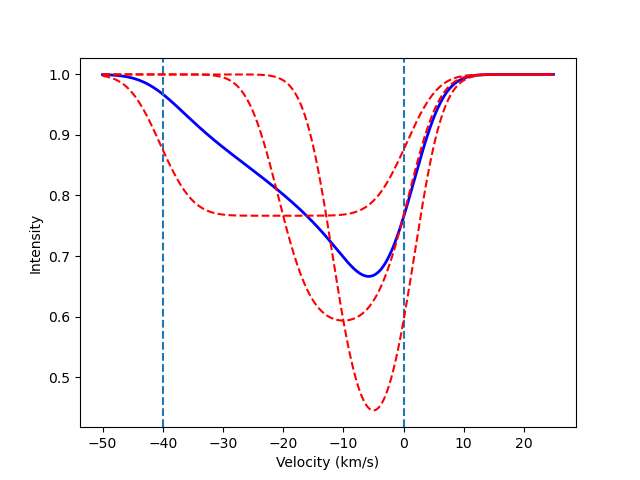
\includegraphics[width=0.5\textwidth]{Figure_1b.png}
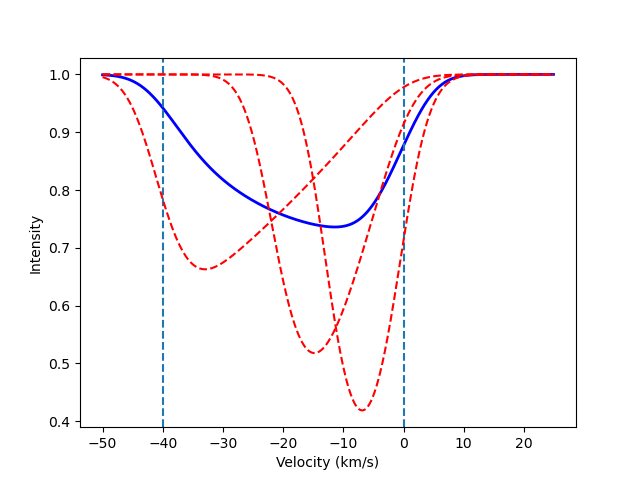
\includegraphics[width=0.5\textwidth]{Figure_1c.png}
\caption{ }
%\includegraphics[width=0.5\textwidth]{mucep_polarization_peaks_limits_v2.png}
%\caption{Velocity position (upper plot) and span (lower plot) of the linear polarization spectral features of $\mu$ Cep over the whole data set of available observations. On the top plot, dots record the position of the signal peaks, while in the bottom plot the vertical lines show the span of signal above noise level. The two horizontal lines in both plots mark the velocity of the center of mass of the star $V_*$ (red line, at +35 \kms) and the maximum velocity of the convecting plasma $V_p$ (blue line, at -35\kms). Velocities are measured in the heliocentric reference system.}
\label{example}
\end{figure*}

Changing the gradients of the velocity along the line of sight, even with no modification of the maximum velocities involved, which is 
always $40km/s$ in the examples of Fig.\ref{example}, we witness dramatic changes in the shape of the profiles. Althoug always asymmetric as computed, the example 
show the path towards narrowing the disk-integrated line profile. Furthermore we see how the bisector can be modified without changing neither the velocities 
. A ballistic drop in velocity near disk center produces a C-shape bisector if it dominates the integrated brightness so that any limb contribution is 
small. But a linear drop in velocity near disk center will produce an inverse C-shape integrated line if the limb contributes with similar brightness to the 
disk integrated profile. The combination of strong gradients of different dependence with $z$, brightness inhomogeneities and disk integration 
appears to be what is needed to reproduce the observed intensity profiles in different RSG.

\section{Reproducing the observed intensity profiles.}

\begin{figure*}
   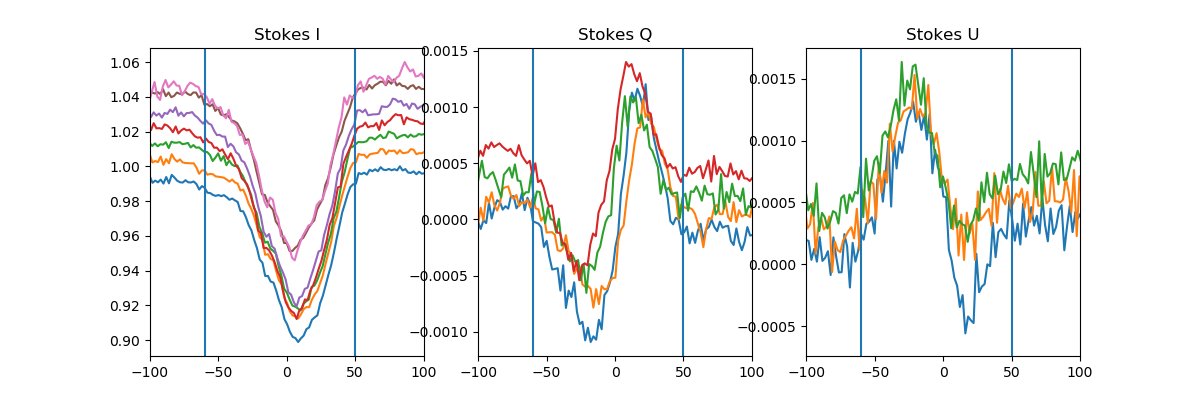
\includegraphics[width=0.8\textwidth]{RWCep.png}
   \caption{ }
   %\includegraphics[width=0.5\textwidth]{mucep_polarization_peaks_limits_v2.png}
   %\caption{Velocity position (upper plot) and span (lower plot) of the linear polarization spectral features of $\mu$ Cep over the whole data set of available observations. On the top plot, dots record the position of the signal peaks, while in the bottom plot the vertical lines show the span of signal above noise level. The two horizontal lines in both plots mark the velocity of the center of mass of the star $V_*$ (red line, at +35 \kms) and the maximum velocity of the convecting plasma $V_p$ (blue line, at -35\kms). Velocities are measured in the heliocentric reference system.}
   \label{observed}
   \end{figure*}

Fig. \ref{observed} shows selected examples of profiles of Betelgeuse and RW Cep, which represent the two extremes of profile shapes 
observed in RSG with Narval and NeoNarval \cite[see][for a description of both instruments and the data reduction procedures]{LA,Donati}.
Betelgeuse profiles date from 2013 and 2014. This data has been presented before by \cite{Auriere}. Though Betelgeuse is being observed periodically 
in recent years, after the great dimming event of the end of 2019 the levels of linear polarisation have drastically diminished. Since 
it is our purpose to illustrate the difference in wavelength span between the linear polarisation and the intensity profile, we have 
preferred the old data to better illustrate the point. Intensity profiles of Betelgeuse keep being in 2023 as narrow as in 2013. For our 
second star, RW Cep, the amplitude of linear polarisation is not an issue in 2023. And therefore we present here NeoNarval data from 
WHICH DATES?. 

We have seen that the presence of velocity gradients larger than the width of the line and of different dependences with $z$ opens the door to a 
variety of profile shapes, from purely gaussian to saw-tooth shapes, from broad to narrow ones. Which one is present in the observation 
of an RSG at a given date depends on the distribution of both gradients and brightness over the disk at the moment of the observation. 
For the sake of simplicity we are going to fix gradients to be of the ballistic kind, with a square root dependence on $z$. But we are going 
to vary both the amplitude of the gradients (changing the parameter $\beta$) and the distribution of brightness and velocity amplitudes over 
the disk. We will select the images inferred from linear polarisation of Betelgeuse to represent what we believe are acceptable 
distributions of brightness and velocities over the disk, recalling that both magnitudes, brightness and velocity, are relied in the 
inversion algorithms fitting linear polarisation as if the light-emitting plasma was in the presence of convection. 

Fig. \ref{betelbeta1} shows the case of $\beta=1$, that is the velocity at each point drops from the value found in the inferred image to zero 
in the span of the formation region of the line. This is quite a large gradient near disk center, with maxximum velocities reaching 
$40 km/s$, but it reduces to a zero gradient towards the limb. The disk-integrated profile will be a combination of saw-tooth and gaussian 
profiles as in Fig.\ref{example}. But the distribution of brighness is not homogeneous, and some profiles will be given more weight 
than others. The result can be seen in Fig. \ref{betelbeta1}.

\begin{figure*}
   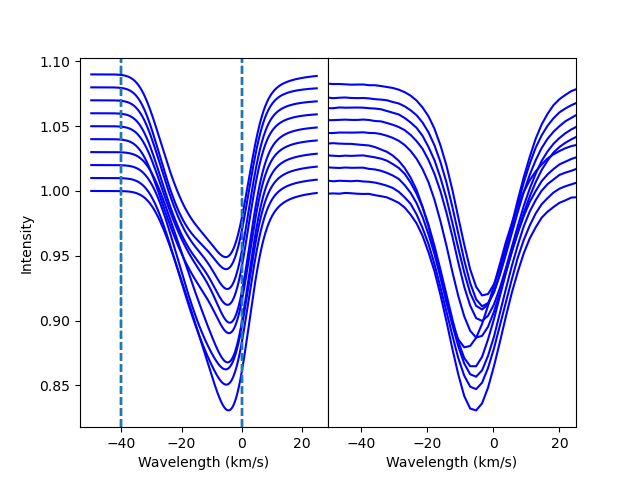
\includegraphics[width=0.8\textwidth]{Fig1_Nadira1.png}
   \caption{ }
   %\includegraphics[width=0.5\textwidth]{mucep_polarization_peaks_limits_v2.png}
   %\caption{Velocity position (upper plot) and span (lower plot) of the linear polarization spectral features of $\mu$ Cep over the whole data set of available observations. On the top plot, dots record the position of the signal peaks, while in the bottom plot the vertical lines show the span of signal above noise level. The two horizontal lines in both plots mark the velocity of the center of mass of the star $V_*$ (red line, at +35 \kms) and the maximum velocity of the convecting plasma $V_p$ (blue line, at -35\kms). Velocities are measured in the heliocentric reference system.}
   \label{betelbeta1}
   \end{figure*}

We have chosen the value of $k$ in \ref{opacityintegral} so that the disk-integrated profile matches the depth of the observed 
intensity profile. Otherwise all parameters are those used by the inversion code to fit the linear polarisation profiles: maximum velocity amplitude and width of the Gaussian profile. The comparison of these so-computed profiles 
and the observed ones is remarkable. The computed profiles are narrow, in spite of the span of velocities used for the computation. This 
is due, as we keep repeating, to the combination of large velocity gradients and the brightness distribution over the disk. The zero velocity
falls in the red wing of the line, consistent with the ad-hoc choice made in the inversion codes. This is an emergent feature, there is 
nothin in the computation that forces the position of the minimum of the disk-integrated profile. The same can be said about the 
maximum velocity, that falls over the continuum well beyond the blue wing of the line, in spite of the presence of large velocities 
at some points over the disk. We conclude from this comparison, that our basic model captures the main features of the observed profiles 
of Betelgeuse. This is in spite of imposing a constant absorption coefficient over the atmosphere, and of imposing the same velocity 
gradient dependence for all points.  We shall look later into the bisector shape and the velocity spans to further push this comparison. 
At this point we can however dare to extract a far-edged conclusion. The model for linear polarisation is based upon the assumption that 
this linear polarization emerges from Rayleigh scattering of the continuum. The continuum polarised photons are subsequently absorbed 
by atoms higher in the atmosphere which re-emit them unpolarised. The local continuum polarisation is in this manner deleted in the spectral line, and it is 
this de-polarisation signal that we measure with our instruments. While the polarization amplitude, in that model is mostly attached 
to the brightness of the continuum emitting plasma, the Doppler shift of the de-polarized photon is that of the absorbing and re-emitting atom. 
Linear polarisation profiles present a broad span  of velocities, but the present comparison of computed and observed intensity 
profiles appears to require a gradient of velocities down to zero over the region of formation of the line. We must conclude 
in consequence that de-polarised photons are coming from the very first lengths of this formation region, while the photons making 
the spectral line come from the integration along the whole region.

RW Cep presents the other end of the variation seen in the intensity profiles of RSG. We see,in the recent observations of this star, 
broadened profiles with a span comparable to the one observed in the linear polarisation profiles. In Fig.\ref{RWbeta} we repeat 
our calculations of disk-integrated profiles with the same brightness distributions used for Betelgeuse (and therefore inferred 
from the fit of the observed linear polarisation of Betelgeuse) but just changing the value of $\beta=0.2$. This value of $\beta$ means 
that rather than dropping to zero along th formation region of the spectral line, the velocity diminishes of just 10\%. With such 
small gradients we recover the flat-bottom profiles that we can favourably compare to the observed profiles of RW Cep. Whenever 
the brightness distribution is such that hot large spots are present over the disk, one can even find split profiles. These are not 
seen in the present observations of RW Cep, but we notice that \cite{Kravchenko} presents observations of another RSG, V Tau, with 
some split line profiles that could be compared to the ones we compute here. 

This second favourable comparison between our simple model and observations gives further support to it. In our view it confirms 
the hypothesis that the geometry of the radiative transfer and, in particular, the combination of the brightness distribution and 
the actual gradients of velocity present at the particular moment of the observation, are sufficient to qualitatively reproduce 
the observed intensity profiles. 

\begin{figure*}
   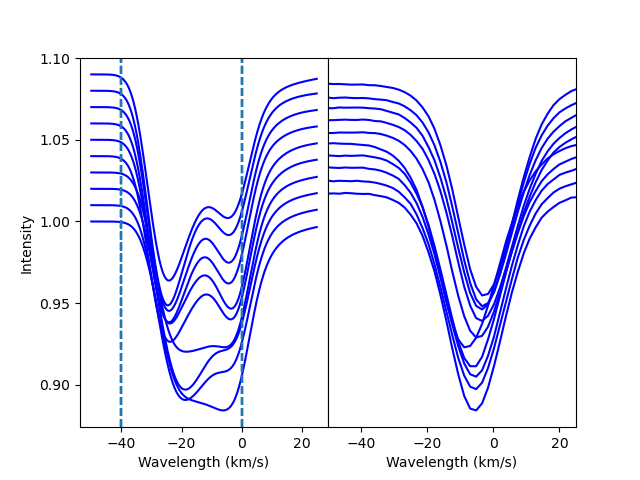
\includegraphics[width=0.8\textwidth]{Fig1_Nadira2.png}
   \caption{ }
   %\includegraphics[width=0.5\textwidth]{mucep_polarization_peaks_limits_v2.png}
   %\caption{Velocity position (upper plot) and span (lower plot) of the linear polarization spectral features of $\mu$ Cep over the whole data set of available observations. On the top plot, dots record the position of the signal peaks, while in the bottom plot the vertical lines show the span of signal above noise level. The two horizontal lines in both plots mark the velocity of the center of mass of the star $V_*$ (red line, at +35 \kms) and the maximum velocity of the convecting plasma $V_p$ (blue line, at -35\kms). Velocities are measured in the heliocentric reference system.}
   \label{RWbeta}
   \end{figure*}

% \begin{figure}
% \includegraphics[width=0.5\textwidth]{FigN.png}
% \caption{Pile-up of the Stokes Q (left), U (center) and I (right) profiles over the whole time series. For illustrative purposes, every observation has been made to span 15 days on the vertical direction. The blue and red vertical lines mark the maximum plasma velocity $V_p$ and the radial velocity of the center of mass of the star $V_*$ respectively (see main text for definitions). Velocities are measured in the heliocentric reference system. }
% %\includegraphics[width=0.5\textwidth]{mucep_polarization_peaks_limits_v2.png}
% %\caption{Velocity position (upper plot) and span (lower plot) of the linear polarization spectral features of $\mu$ Cep over the whole data set of available observations. On the top plot, dots record the position of the signal peaks, while in the bottom plot the vertical lines show the span of signal above noise level. The two horizontal lines in both plots mark the velocity of the center of mass of the star $V_*$ (red line, at +35 \kms) and the maximum velocity of the convecting plasma $V_p$ (blue line, at -35\kms). Velocities are measured in the heliocentric reference system.}
% \label{velos}
% \end{figure}

\section{Bisectors and velocity span}

Observed isectors bring up harder constraints into the line formation process. Figs. \ref{couche6} and \ref{couche0} show the measured 
bisectors on intensite profiles of Betelgeuse in the period XXXX. In Fig. \ref{couche6} intensity profiles are made with a line mask 
that selects lines formed in the upper part of the atmosphere. This mask was selected and created by \cite{Kravchenko}. Strongly curved 
inverse C-shape bisectors are seen in the lines formed in this top photospheric layer, a feature traditionally interpreted as the 
presence of accelerating rising plasma.   In Fig. \ref{couche0} lines formed deeper in the photosphere have been selected, by the simplest 
procedure of selecting lines with central depressions in the range of 0.6 to 0.7 the continuum intensity. In these deepest layers, and 
for all the periods observed, the bisectors are straight with a tendency to bend towards the red in the top parts in what looks as 
the more common C-shape bisectors.
\begin{figure*}
   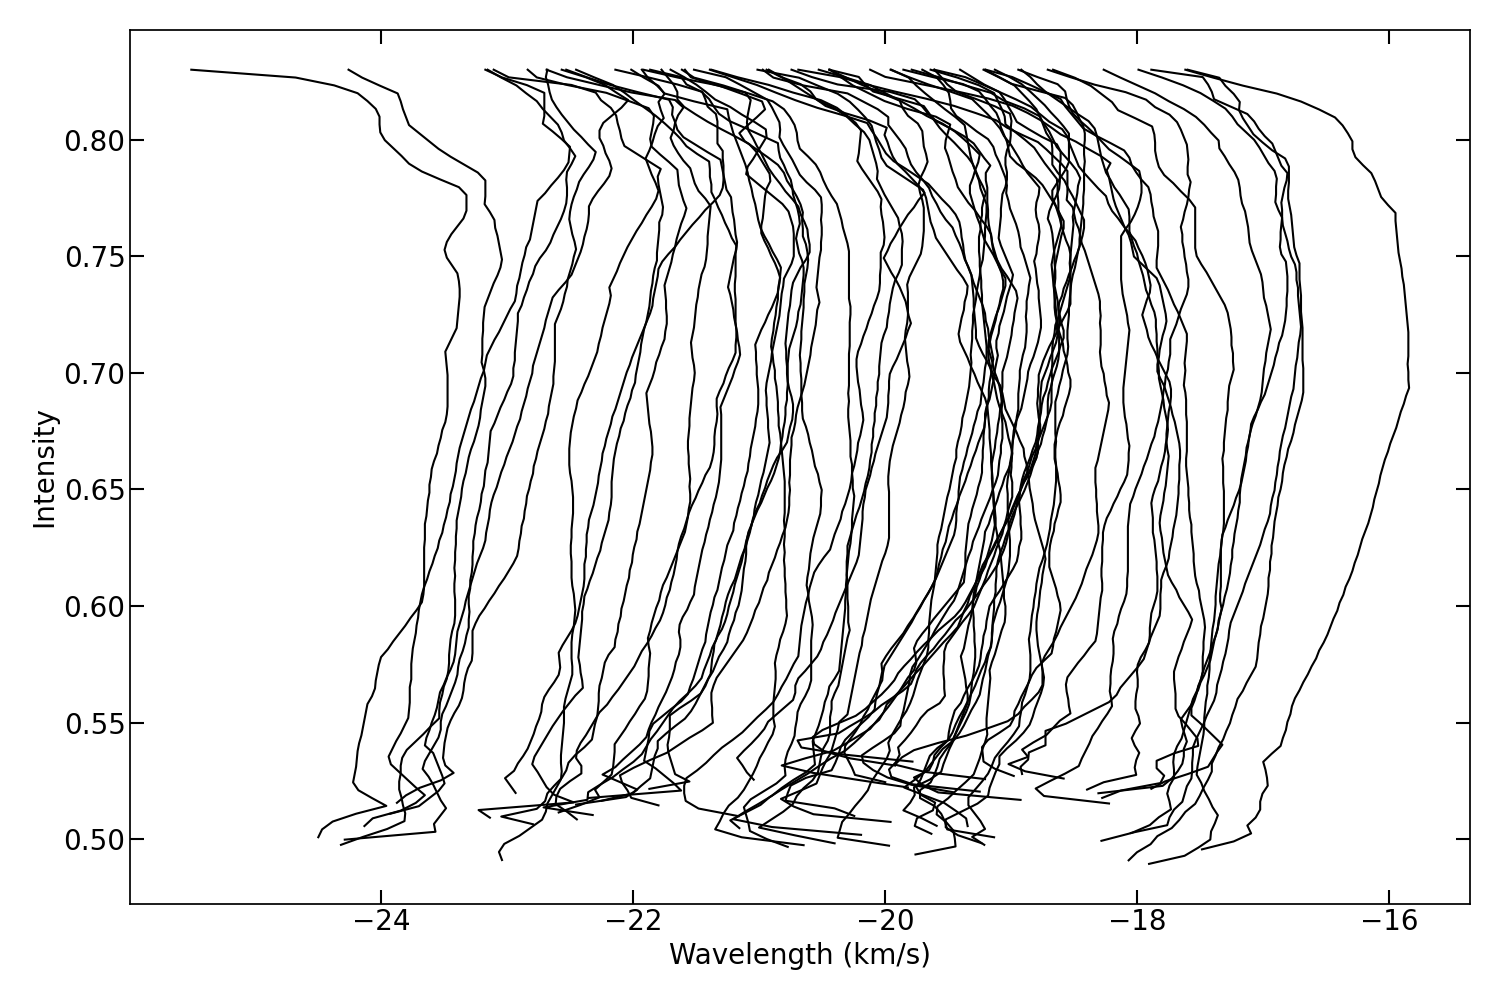
\includegraphics[width=0.8\textwidth]{bissecteurmaskKateryna.png}
   \caption{ }
   %\includegraphics[width=0.5\textwidth]{mucep_polarization_peaks_limits_v2.png}
   %\caption{Velocity position (upper plot) and span (lower plot) of the linear polarization spectral features of $\mu$ Cep over the whole data set of available observations. On the top plot, dots record the position of the signal peaks, while in the bottom plot the vertical lines show the span of signal above noise level. The two horizontal lines in both plots mark the velocity of the center of mass of the star $V_*$ (red line, at +35 \kms) and the maximum velocity of the convecting plasma $V_p$ (blue line, at -35\kms). Velocities are measured in the heliocentric reference system.}
   \label{couche0}
   \end{figure*}
   \begin{figure*}
      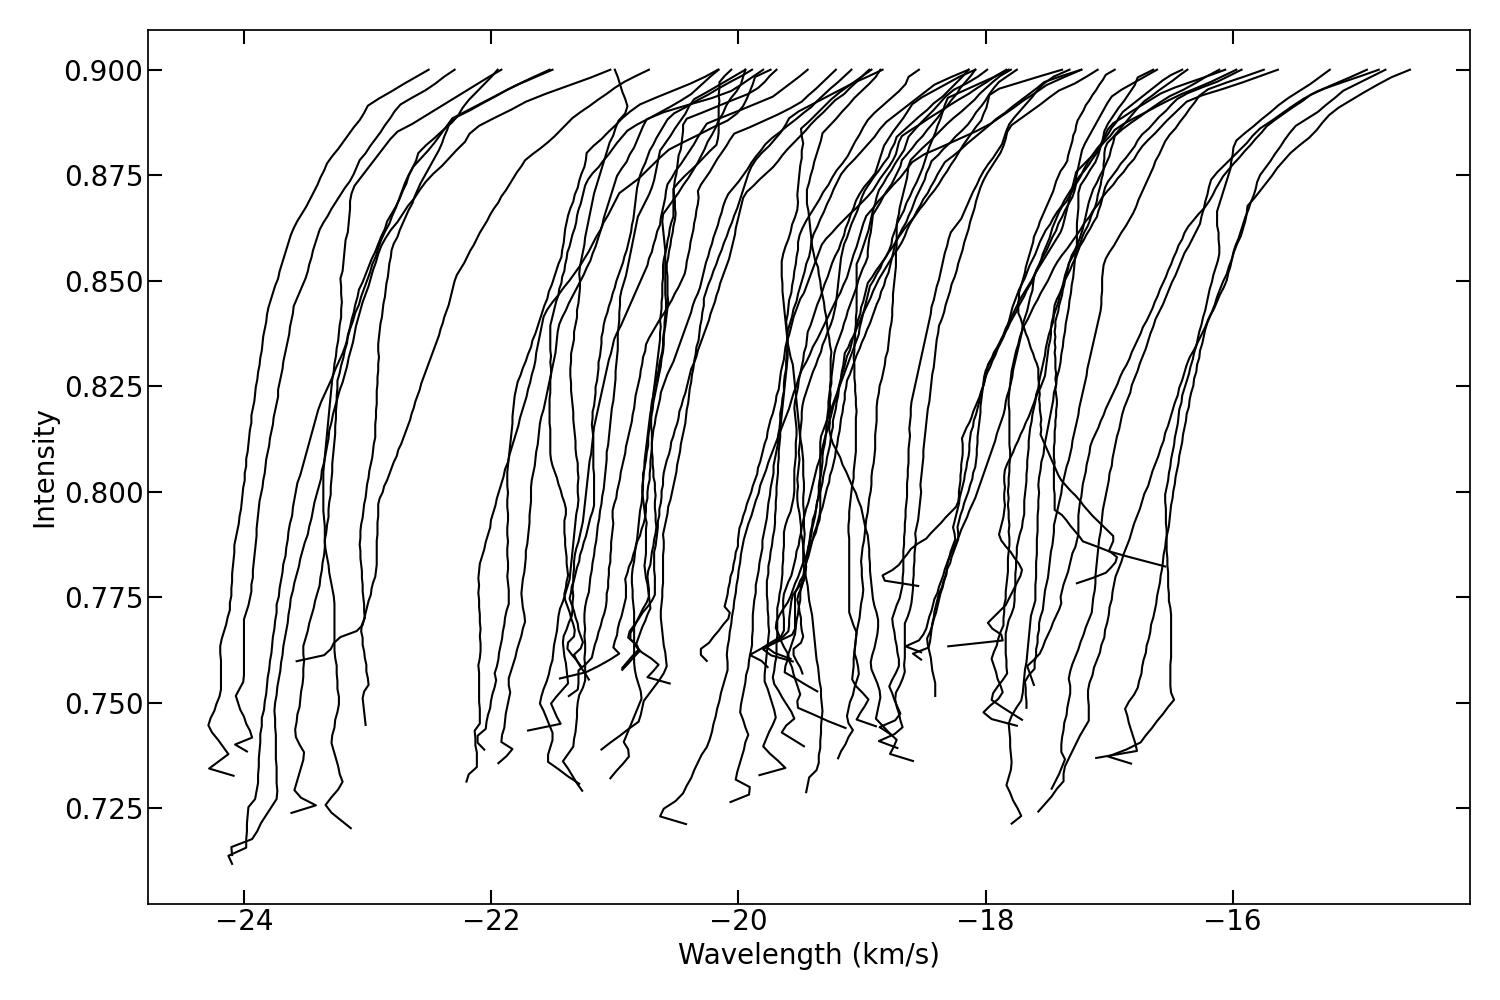
\includegraphics[width=0.8\textwidth]{bissecteurcouche06_07.png}
      \caption{ }
      %\includegraphics[width=0.5\textwidth]{mucep_polarization_peaks_limits_v2.png}
      %\caption{Velocity position (upper plot) and span (lower plot) of the linear polarization spectral features of $\mu$ Cep over the whole data set of available observations. On the top plot, dots record the position of the signal peaks, while in the bottom plot the vertical lines show the span of signal above noise level. The two horizontal lines in both plots mark the velocity of the center of mass of the star $V_*$ (red line, at +35 \kms) and the maximum velocity of the convecting plasma $V_p$ (blue line, at -35\kms). Velocities are measured in the heliocentric reference system.}
      \label{couche6}
      \end{figure*}
   

\begin{figure*}
   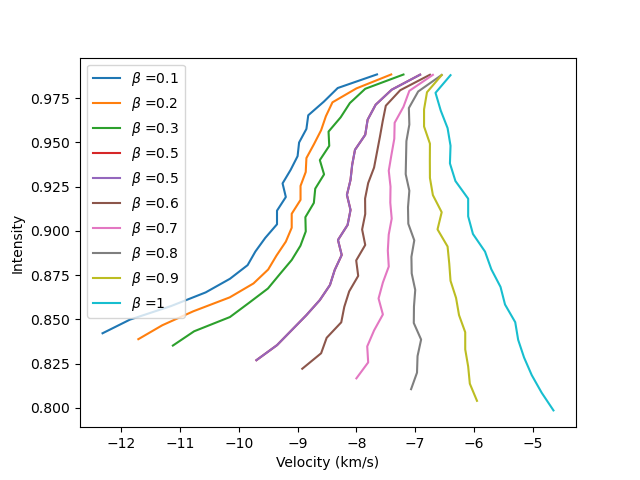
\includegraphics[width=0.8\textwidth]{Bisectors_cual1.png}
   \caption{ }
   %\includegraphics[width=0.5\textwidth]{mucep_polarization_peaks_limits_v2.png}
   \caption{cual=1, vels*0.7}
   \label{bisector1}
   \end{figure*}


Reproducing not just the width of the profile, as done in the previous section, but also the bisector asymmetry is harder with such 
a simple radiative transfer as we are here limiting ourselves. The presence of strong gradients was seen as a requirement to make 
compatible the broad linear polarisation profiles and the narrow intensity profiles of Betelgeuse, while reducing them was the key 
to also explain RW Cep profiles. This main conclusion also applies when trying to reproduce bisectors. Fig. \ref{bisector1} shows 
the bisectors of disk-integrated profiles using the inferred image of Betelgeuse for the date of XXXX. While the square root gradient 
is used in all the cases, the value of $\beta$ is changed to simulate almost no gradient ($\beta=0.1$) to a full decrease to zero 
velocity ($\beta=1$). Affording very low gradients while maintaining the gaussian shape of Betelgeuse profiles and not drifting towards 
RW Cep-like profiles requires reducing the maximum velocities to 70\% the original values. With this difference taken into account, 
the computed bisectors can be favourably compared to the observed ones of Fig.\ref{couche6}, particuler for values of $\beta~0.5$. 
Such lower values of $\beta$ may be justified by the smaller region covered by the formation region of these lines. But one must 
not over-interpret the comparison of real data with such a simple radiative transfer problem. The important conclusion is that 
observed bisectors are still sufficiently well reproduced by the simple model requiring strong gradients and the actual plasma velocities 
and brightness inhomogeneities inferred from the fit of the linear polarisation profiles. 

The top photospheric layers present a pronouncedly inverse C-shape at all dates. These lines sometimes dominate the total line 
made of the addition of all lines, which explains that the bisector at some dates presents an inverse C-shape while more often 
presents a normal C-shape. But when isolated in separate layers, the bisector maintains its shape at all dates. This inverse C-shape 
is traditionally interpreted as the presence of accelerating and rising plasma. And so appears to be the case in our simple model 
as well. And to reproduce these bisectors we need to abandon the square root decerease in velocity and use a gradient that increases 
the velocity linearly as $v(z)=v_0\beta z$. The resulting bisectors can be seen in  Fig. \ref{bisector2}. For constant velocities 
($\beta=0.1$) the bisector is almos straigth. As the gradient increeases and, particularly, for $\beta >1$ inverse C-shape bisectors 
appear. These do not reproduce completely the observed bisectors of Fig.\ref{couche0}. One is tempted to suggest that the lines 
of this upper photosphere start forming while negative gradients are still present, but that it is in mid formation region that 
the actual acceleration appears. 


\begin{figure*}
   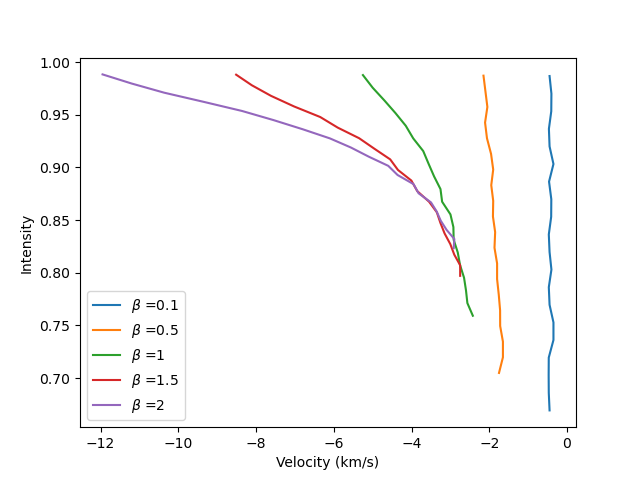
\includegraphics[width=0.8\textwidth]{Bisectors_accel.png}
   \caption{ }
   %\includegraphics[width=0.5\textwidth]{mucep_polarization_peaks_limits_v2.png}
   \caption{$v(z)=v_0\beta z$}
   \label{bisector2}
   \end{figure*}

\section{Conclusion}


\begin{acknowledgements}
This work was supported by the "Programme National de Physique Stellaire" (PNPS) of CNRS/INSU co-funded by CEA and CNES.
\end{acknowledgements}

\bibliographystyle{/Users/art2/TeX/aanda/bibtex/aa}
%\bibliographystyle{aa}

\bibliography{art74}

 

\end{document} 
